\documentclass[convert={size=640}]{standalone}
\usepackage{tikz}
\usetikzlibrary{arrows}
\usetikzlibrary{arrows.meta}
\usetikzlibrary{shadows}
\usetikzlibrary{positioning}
\usetikzlibrary{calc}
\usetikzlibrary{backgrounds}

\begin{document}

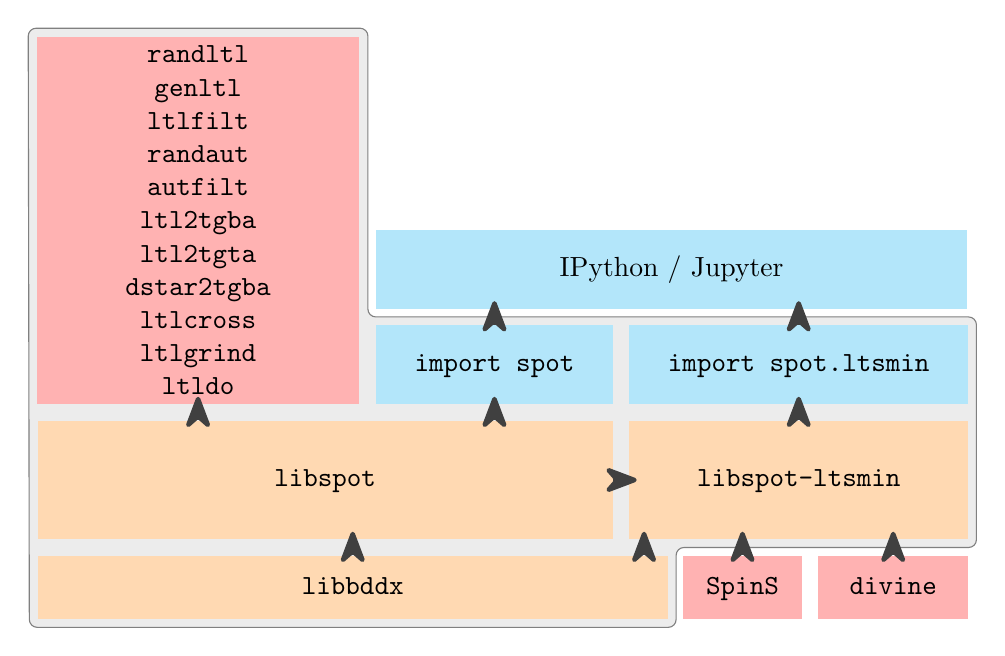
\begin{tikzpicture}
  \tikzset{cppbox/.style={minimum width=#1,fill=orange!30, minimum height=1.5cm},
           pybox/.style={minimum width=#1,fill=cyan!30, minimum height=1cm},
           shbox/.style={minimum width=#1,fill=red!30, minimum height=8mm},
           usedby/.style={->,ultra thick,>={Stealth[length=5mm,round]},gray!50!black}}
  \node[cppbox=7.3cm] (libspot) {\texttt{libspot\strut}};
  \node[cppbox=4.3cm,right=2mm]
     (libltsmin) at (libspot.east) {\texttt{libspot-ltsmin\strut}};
  \node[cppbox=8cm,below right,yshift=-2mm,minimum height=8mm] (buddy) at (libspot.south west) {\texttt{libbddx\strut}};

  \node[pybox=4.3cm,above=2mm] (pyltsmin) at (libltsmin.north) {\texttt{import spot.ltsmin\strut}};
  \node[pybox=3cm,left=2mm] (pyspot) at (pyltsmin.west) {\texttt{import spot\strut}};
  \node[shbox=4.1cm,above left,xshift=-2mm,align=center] (shcmd) at (pyspot.south west) {
    \texttt{randltl}\\
    \texttt{genltl}\\
    \texttt{ltlfilt}\\
    \texttt{randaut}\\
    \texttt{autfilt}\\
    \texttt{ltl2tgba}\\
    \texttt{ltl2tgta}\\
    \texttt{dstar2tgba}\\
    \texttt{ltlcross}\\
    \texttt{ltlgrind}\\
    \texttt{ltldo}
  };
  \node[shbox=1.9cm,below left,yshift=-2mm] (divine) at (libltsmin.south east) {\texttt{divine\strut}};
  \node[shbox=1.5cm,left,xshift=-2mm] (spins) at (divine.west) {\texttt{SpinS\strut}};
  \node[pybox=7.5cm,above right,yshift=2mm] (ipython) at (pyspot.north west) {IPython / Jupyter};
  \draw[usedby] (buddy.north) -- ++(0,3mm);
  \draw[usedby] (buddy.north) ++(3.7cm,0) -- ++(0,3mm);
  \draw[usedby] (spins.north) -- ++(0,3mm);
  \draw[usedby] (divine.north) -- ++(0,3mm);
  \draw[usedby] (libspot.east) -- ++(3mm,0);
  \draw[usedby] (pyspot.south) ++(0,-2mm) -- ++(0,3mm);
  \draw[usedby] (pyltsmin.south) ++(0,-2mm) -- ++(0,3mm);
  \draw[usedby] (shcmd.south) ++(0,-2mm) -- ++(0,3mm);
  \draw[usedby] (pyspot.north) -- ++(0,3mm);
  \draw[usedby] (pyltsmin.north) -- ++(0,3mm);

  \begin{pgfonlayer}{background}
  \path[fill=gray!15,draw=gray,rounded corners=1mm]
  ($(shcmd.north west)+(-1mm,1mm)$) --
  ($(shcmd.north east)+(1mm,1mm)$) --
  ($(pyspot.north west)+(-1mm,1mm)$) --
  ($(pyltsmin.north east)+(1mm,1mm)$) --
  ($(libltsmin.south east)+(1mm,-1mm)$) --
  ($(buddy.north east)+(1mm,1mm)$) --
  ($(buddy.south east)+(1mm,-1mm)$) --
  ($(buddy.south west)+(-1mm,-1mm)$) -- cycle;
  \end{pgfonlayer}
\end{tikzpicture}
\end{document}
%%% Local Variables:
%%% mode: latex
%%% TeX-master: t
%%% End:
